% Options for packages loaded elsewhere
% Options for packages loaded elsewhere
\PassOptionsToPackage{unicode}{hyperref}
\PassOptionsToPackage{hyphens}{url}
\PassOptionsToPackage{dvipsnames,svgnames,x11names}{xcolor}
%
\documentclass[
  letterpaper,
  DIV=11,
  numbers=noendperiod]{scrartcl}
\usepackage{xcolor}
\usepackage{amsmath,amssymb}
\setcounter{secnumdepth}{-\maxdimen} % remove section numbering
\usepackage{iftex}
\ifPDFTeX
  \usepackage[T1]{fontenc}
  \usepackage[utf8]{inputenc}
  \usepackage{textcomp} % provide euro and other symbols
\else % if luatex or xetex
  \usepackage{unicode-math} % this also loads fontspec
  \defaultfontfeatures{Scale=MatchLowercase}
  \defaultfontfeatures[\rmfamily]{Ligatures=TeX,Scale=1}
\fi
\usepackage{lmodern}
\ifPDFTeX\else
  % xetex/luatex font selection
\fi
% Use upquote if available, for straight quotes in verbatim environments
\IfFileExists{upquote.sty}{\usepackage{upquote}}{}
\IfFileExists{microtype.sty}{% use microtype if available
  \usepackage[]{microtype}
  \UseMicrotypeSet[protrusion]{basicmath} % disable protrusion for tt fonts
}{}
\makeatletter
\@ifundefined{KOMAClassName}{% if non-KOMA class
  \IfFileExists{parskip.sty}{%
    \usepackage{parskip}
  }{% else
    \setlength{\parindent}{0pt}
    \setlength{\parskip}{6pt plus 2pt minus 1pt}}
}{% if KOMA class
  \KOMAoptions{parskip=half}}
\makeatother
% Make \paragraph and \subparagraph free-standing
\makeatletter
\ifx\paragraph\undefined\else
  \let\oldparagraph\paragraph
  \renewcommand{\paragraph}{
    \@ifstar
      \xxxParagraphStar
      \xxxParagraphNoStar
  }
  \newcommand{\xxxParagraphStar}[1]{\oldparagraph*{#1}\mbox{}}
  \newcommand{\xxxParagraphNoStar}[1]{\oldparagraph{#1}\mbox{}}
\fi
\ifx\subparagraph\undefined\else
  \let\oldsubparagraph\subparagraph
  \renewcommand{\subparagraph}{
    \@ifstar
      \xxxSubParagraphStar
      \xxxSubParagraphNoStar
  }
  \newcommand{\xxxSubParagraphStar}[1]{\oldsubparagraph*{#1}\mbox{}}
  \newcommand{\xxxSubParagraphNoStar}[1]{\oldsubparagraph{#1}\mbox{}}
\fi
\makeatother


\usepackage{longtable,booktabs,array}
\newcounter{none} % for unnumbered tables
\usepackage{calc} % for calculating minipage widths
% Correct order of tables after \paragraph or \subparagraph
\usepackage{etoolbox}
\makeatletter
\patchcmd\longtable{\par}{\if@noskipsec\mbox{}\fi\par}{}{}
\makeatother
% Allow footnotes in longtable head/foot
\IfFileExists{footnotehyper.sty}{\usepackage{footnotehyper}}{\usepackage{footnote}}
\makesavenoteenv{longtable}
\usepackage{graphicx}
\makeatletter
\newsavebox\pandoc@box
\newcommand*\pandocbounded[1]{% scales image to fit in text height/width
  \sbox\pandoc@box{#1}%
  \Gscale@div\@tempa{\textheight}{\dimexpr\ht\pandoc@box+\dp\pandoc@box\relax}%
  \Gscale@div\@tempb{\linewidth}{\wd\pandoc@box}%
  \ifdim\@tempb\p@<\@tempa\p@\let\@tempa\@tempb\fi% select the smaller of both
  \ifdim\@tempa\p@<\p@\scalebox{\@tempa}{\usebox\pandoc@box}%
  \else\usebox{\pandoc@box}%
  \fi%
}
% Set default figure placement to htbp
\def\fps@figure{htbp}
\makeatother





\setlength{\emergencystretch}{3em} % prevent overfull lines

\providecommand{\tightlist}{%
  \setlength{\itemsep}{0pt}\setlength{\parskip}{0pt}}



 


\KOMAoption{captions}{tableheading}
\makeatletter
\@ifpackageloaded{caption}{}{\usepackage{caption}}
\AtBeginDocument{%
\ifdefined\contentsname
  \renewcommand*\contentsname{Table of contents}
\else
  \newcommand\contentsname{Table of contents}
\fi
\ifdefined\listfigurename
  \renewcommand*\listfigurename{List of Figures}
\else
  \newcommand\listfigurename{List of Figures}
\fi
\ifdefined\listtablename
  \renewcommand*\listtablename{List of Tables}
\else
  \newcommand\listtablename{List of Tables}
\fi
\ifdefined\figurename
  \renewcommand*\figurename{Figure}
\else
  \newcommand\figurename{Figure}
\fi
\ifdefined\tablename
  \renewcommand*\tablename{Table}
\else
  \newcommand\tablename{Table}
\fi
}
\@ifpackageloaded{float}{}{\usepackage{float}}
\floatstyle{ruled}
\@ifundefined{c@chapter}{\newfloat{codelisting}{h}{lop}}{\newfloat{codelisting}{h}{lop}[chapter]}
\floatname{codelisting}{Listing}
\newcommand*\listoflistings{\listof{codelisting}{List of Listings}}
\makeatother
\makeatletter
\makeatother
\makeatletter
\@ifpackageloaded{caption}{}{\usepackage{caption}}
\@ifpackageloaded{subcaption}{}{\usepackage{subcaption}}
\makeatother
\usepackage{bookmark}
\IfFileExists{xurl.sty}{\usepackage{xurl}}{} % add URL line breaks if available
\urlstyle{same}
\hypersetup{
  pdftitle={Türkiye'de Sinema Sektörünün Veri Analizi},
  colorlinks=true,
  linkcolor={blue},
  filecolor={Maroon},
  citecolor={Blue},
  urlcolor={Blue},
  pdfcreator={LaTeX via pandoc}}


\title{Türkiye'de Sinema Sektörünün Veri Analizi}
\author{}
\date{}
\begin{document}
\maketitle


\section{Proje Kapsamı}\label{proje-kapsamux131}

Türkiye sinema sektörünün yıllara göre değişimi incelenmiştir. Sinema
salonu sayıları, gösterilen film sayıları ve seyirci eğilimleri analiz
edilmiştir.

\section{Grup Üyeleri}\label{grup-uxfcyeleri}

Ceren -pagelink-

Esin -pagelink-

Baran -pagelink-

\section{Veri}\label{veri}

\begin{longtable}[]{@{}
  >{\raggedleft\arraybackslash}p{(\linewidth - 16\tabcolsep) * \real{0.0318}}
  >{\raggedleft\arraybackslash}p{(\linewidth - 16\tabcolsep) * \real{0.0892}}
  >{\raggedleft\arraybackslash}p{(\linewidth - 16\tabcolsep) * \real{0.0892}}
  >{\raggedleft\arraybackslash}p{(\linewidth - 16\tabcolsep) * \real{0.1465}}
  >{\raggedleft\arraybackslash}p{(\linewidth - 16\tabcolsep) * \real{0.1401}}
  >{\raggedleft\arraybackslash}p{(\linewidth - 16\tabcolsep) * \real{0.1529}}
  >{\raggedleft\arraybackslash}p{(\linewidth - 16\tabcolsep) * \real{0.0955}}
  >{\raggedleft\arraybackslash}p{(\linewidth - 16\tabcolsep) * \real{0.1210}}
  >{\raggedleft\arraybackslash}p{(\linewidth - 16\tabcolsep) * \real{0.1338}}@{}}
\caption{Düzenlenmiş Veri Seti}\tabularnewline
\toprule\noalign{}
\begin{minipage}[b]{\linewidth}\raggedleft
yil
\end{minipage} & \begin{minipage}[b]{\linewidth}\raggedleft
sinema\_salonu
\end{minipage} & \begin{minipage}[b]{\linewidth}\raggedleft
koltuk\_sayisi
\end{minipage} & \begin{minipage}[b]{\linewidth}\raggedleft
gosterilen\_film\_toplam
\end{minipage} & \begin{minipage}[b]{\linewidth}\raggedleft
gosterilen\_yerli\_film
\end{minipage} & \begin{minipage}[b]{\linewidth}\raggedleft
gosterilen\_yabanci\_film
\end{minipage} & \begin{minipage}[b]{\linewidth}\raggedleft
toplam\_seyirci
\end{minipage} & \begin{minipage}[b]{\linewidth}\raggedleft
yerli\_film\_seyirci
\end{minipage} & \begin{minipage}[b]{\linewidth}\raggedleft
yabanci\_film\_seyirci
\end{minipage} \\
\midrule\noalign{}
\endfirsthead
\toprule\noalign{}
\begin{minipage}[b]{\linewidth}\raggedleft
yil
\end{minipage} & \begin{minipage}[b]{\linewidth}\raggedleft
sinema\_salonu
\end{minipage} & \begin{minipage}[b]{\linewidth}\raggedleft
koltuk\_sayisi
\end{minipage} & \begin{minipage}[b]{\linewidth}\raggedleft
gosterilen\_film\_toplam
\end{minipage} & \begin{minipage}[b]{\linewidth}\raggedleft
gosterilen\_yerli\_film
\end{minipage} & \begin{minipage}[b]{\linewidth}\raggedleft
gosterilen\_yabanci\_film
\end{minipage} & \begin{minipage}[b]{\linewidth}\raggedleft
toplam\_seyirci
\end{minipage} & \begin{minipage}[b]{\linewidth}\raggedleft
yerli\_film\_seyirci
\end{minipage} & \begin{minipage}[b]{\linewidth}\raggedleft
yabanci\_film\_seyirci
\end{minipage} \\
\midrule\noalign{}
\endhead
\bottomrule\noalign{}
\endlastfoot
2000 & 606 & 200853 & 24096 & 4733 & 19363 & 17086152 & 2899103 &
14187049 \\
2001 & 580 & 139664 & 25608 & 5042 & 20566 & 16905737 & 3289438 &
13616299 \\
2002 & 532 & 134045 & 22529 & 3302 & 19227 & 15406597 & 2079671 &
13326926 \\
2003 & 826 & 141839 & 21254 & 3351 & 17903 & 14503052 & 2923286 &
11579766 \\
2004 & 822 & 145298 & 26398 & 4989 & 21409 & 18670834 & 6657156 &
12013678 \\
2005 & 987 & 152234 & 25076 & 5671 & 19405 & 18001466 & 6795791 &
11205675 \\
\end{longtable}

\section{Yıllara Göre Toplam Seyirci Sayısı
Grafiği}\label{yux131llara-guxf6re-toplam-seyirci-sayux131sux131-grafiux11fi}

\pandocbounded{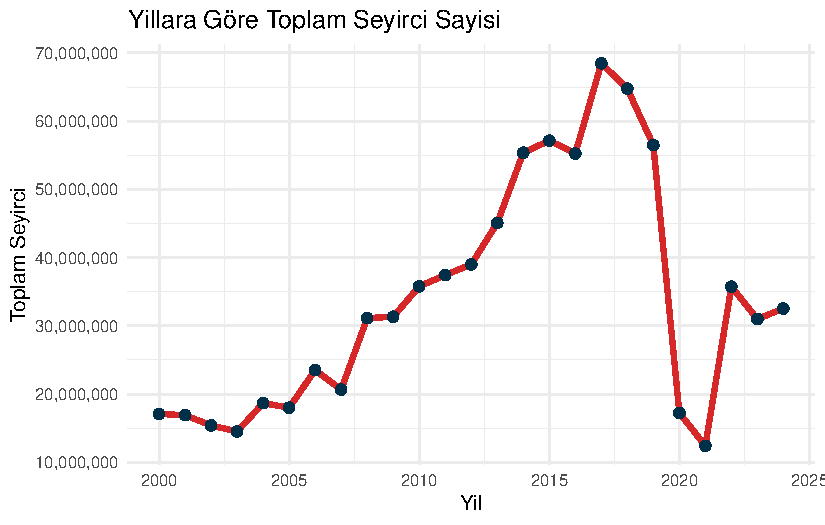
\includegraphics[keepaspectratio]{proje_files/figure-pdf/unnamed-chunk-4-1.pdf}}

Grafik incelendiğinde toplam seyirci sayısının yıllar içerisinde artışta
olduğu görülmektedir.

Özellikle 2020 yılında COVID-19 etkisiyle ciddi bir düşüş yaşanmıştır.

Pandemi sonrası dönemde ise sektör yeniden toparlanma eğilimi
göstermiştir.

\section{Yerli ve Yabancı Film
Analizi}\label{yerli-ve-yabancux131-film-analizi}

\pandocbounded{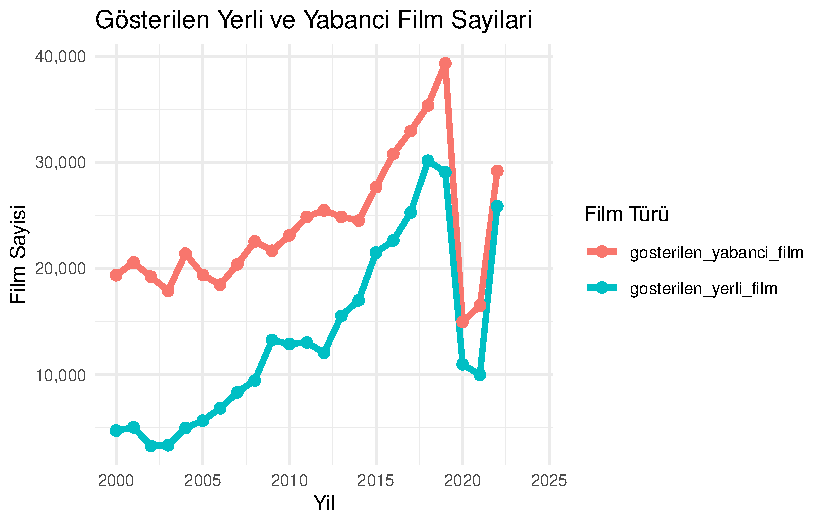
\includegraphics[keepaspectratio]{proje_files/figure-pdf/unnamed-chunk-5-1.pdf}}

Grafik incelendiğinde yabancı film sayısının çoğu dönemde yerli film
sayısından daha yüksek olduğu görülmektedir. Ancak yıllar içerisinde
yerli film sayısında belirgin bir artış yaşanmıştır. Özellikle 2015
sonrası dönemde yerli yapımların sinema sektöründe daha güçlü bir konuma
geldiği dikkat çekmektedir.

\section{COVID-19 Pandeminin Etkisi}\label{covid-19-pandeminin-etkisi}

\pandocbounded{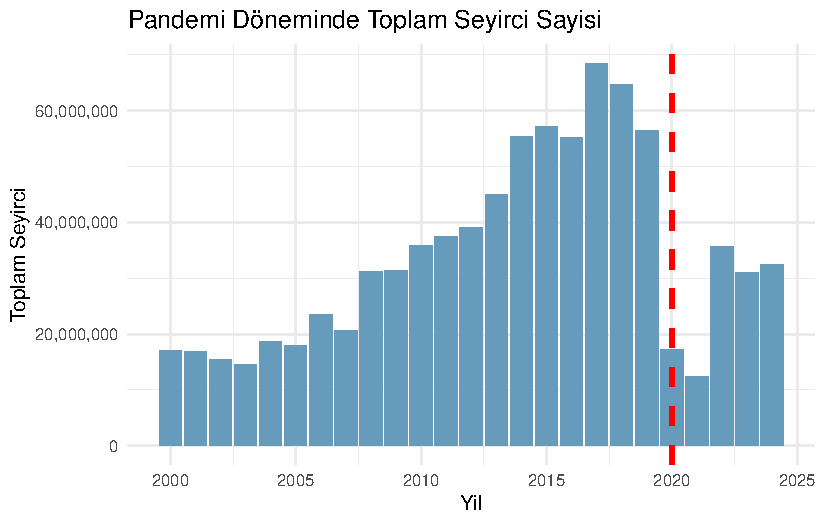
\includegraphics[keepaspectratio]{proje_files/figure-pdf/unnamed-chunk-6-1.pdf}}

2020 yılı sinema sektörü açısından önemli bir kırılma noktasıdır.
COVID-19 nedeniyle sinema salonlarının kapanması ve sosyal kısıtlamalar,
toplam seyirci sayısında belirgin bir düşüşe neden olmuştur. 2021
sonrası dönemde toparlanma eğilimi görülse de dijital platformların
gelişimi sektörün pandemi öncesi seviyelere ulaşmasını zorlaştırmıştır.

\section{Değişkenler Arası
İlişki}\label{deux11fiux15fkenler-arasux131-iliux15fki}

Analiz sonuçları sinema salonu sayısı, koltuk kapasitesi ve toplam
seyirci sayısı arasında pozitif yönlü ilişkiler bulunduğunu
göstermektedir. Özellikle toplam seyirci sayısı ile yerli ve yabancı
film seyircileri arasında güçlü ilişki olduğu gözlemlenmiştir.

\section{Gelecek Yıllara Yönelik Tahmin
Analizi}\label{gelecek-yux131llara-yuxf6nelik-tahmin-analizi}

Bu bölümde toplam seyirci sayısının gelecekteki eğilimini incelemek
amacıyla basit zaman serisi tahmin analizi uygulanmıştır.

\pandocbounded{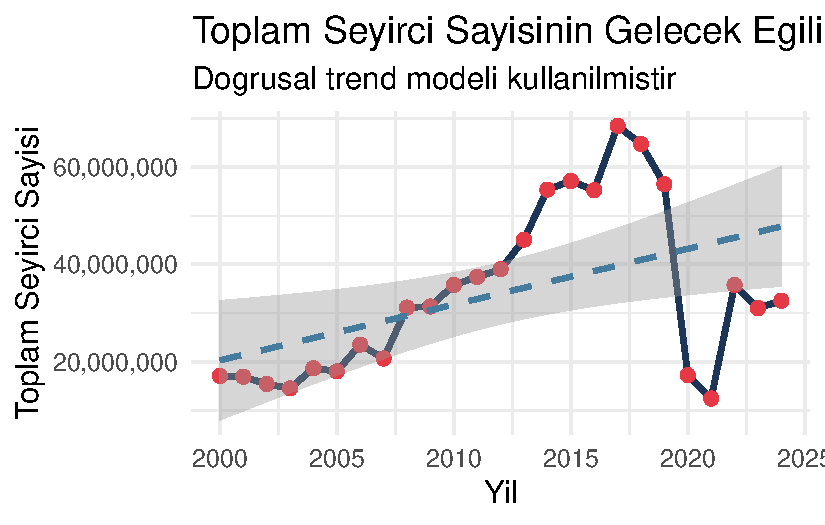
\includegraphics[keepaspectratio]{proje_files/figure-pdf/unnamed-chunk-7-1.pdf}}

\subsection{3.1 Data Source}\label{data-source}

xxxxxx

\subsection{3.2 General Information About
Data}\label{general-information-about-data}

xxxxxx

\subsection{3.3 Reason of Choice}\label{reason-of-choice}

xxxxxx

\subsection{3.4 Preprocessing}\label{preprocessing}

xxxxxx

\section{4. Analysis}\label{analysis}

xxxxxx

\subsection{4.1 Exploratory Data
Analysis}\label{exploratory-data-analysis}

xxxxxx

\subsection{4.2 Trend Analysis}\label{trend-analysis}

xxxxxx

\subsection{4.3 Model Fitting}\label{model-fitting}

xxxxxx

\subsection{4.4 Results}\label{results}

xxxxxx

\section{5. Results and Key Takeaways}\label{results-and-key-takeaways}

xxxxxx




\end{document}
